% The Sauer--Shelah bound as a surface over (n,d), with the admissible curve d = d(n).
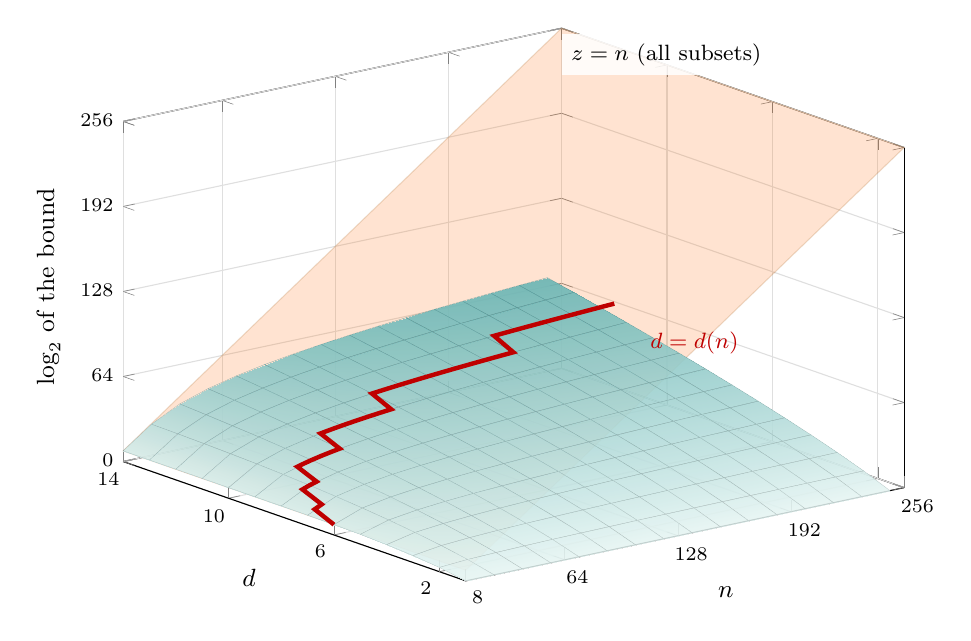
\begin{tikzpicture}
  \begin{axis}[
      width=11.5cm, height=8.6cm,
      view={-38}{24},
      xlabel={$n$}, ylabel={$d$}, zlabel={$\log_2$ of the bound},
      xmin=8, xmax=256, ymin=1, ymax=14, zmin=0, zmax=256,
      xtick={8,64,128,192,256}, ytick={2,6,10,14}, ztick={0,64,128,192,256},
      tick label style={font=\scriptsize}, label style={font=\small},
      grid=major, grid style={gray!25},
      colormap={teal}{rgb255=(230,245,243) rgb255=(0,128,128) rgb255=(10,60,70)},
      z buffer=sort, clip=false]
    % the trivial bound 2^n: the plane z = n
    \addplot3[surf, shader=flat, opacity=0.18, fill=orange!80!red, draw=orange!60!black,
      samples=2, domain=8:256, y domain=1:14] {x};
    % the surface log2 sum_{j<d} binom(n,j)
    \addplot3[surf, shader=faceted interp, opacity=0.9, draw=black!30, line width=0.1pt] table {
8 1 0.000
24 1 0.000
40 1 0.000
56 1 0.000
72 1 0.000
88 1 0.000
104 1 0.000
120 1 0.000
136 1 0.000
152 1 0.000
168 1 0.000
184 1 0.000
200 1 0.000
216 1 0.000
232 1 0.000
248 1 0.000

8 2 3.170
24 2 4.644
40 2 5.358
56 2 5.833
72 2 6.190
88 2 6.476
104 2 6.714
120 2 6.919
136 2 7.098
152 2 7.257
168 2 7.401
184 2 7.531
200 2 7.651
216 2 7.762
232 2 7.864
248 2 7.960

8 3 5.209
24 3 8.234
40 3 9.681
56 3 10.641
72 3 11.360
88 3 11.936
104 3 12.415
120 3 12.826
136 3 13.186
152 3 13.505
168 3 13.793
184 3 14.055
200 3 14.295
216 3 14.517
232 3 14.722
248 3 14.914

8 4 6.539
24 4 11.183
40 4 13.385
56 4 14.839
72 4 15.926
88 4 16.794
104 4 17.517
120 4 18.136
136 4 18.678
152 4 19.159
168 4 19.592
184 4 19.986
200 4 20.347
216 4 20.680
232 4 20.989
248 4 21.278

8 5 7.349
24 5 13.661
40 5 16.639
56 5 18.597
72 5 20.057
88 5 21.222
104 5 22.190
120 5 23.019
136 5 23.744
152 5 24.388
168 5 24.968
184 5 25.494
200 5 25.976
216 5 26.422
232 5 26.835
248 5 27.220

8 6 7.775
24 6 15.759
40 6 19.536
56 6 22.008
72 6 23.846
88 6 25.311
104 6 26.528
120 6 27.569
136 6 28.478
152 6 29.286
168 6 30.012
184 6 30.672
200 6 31.277
216 6 31.835
232 6 32.352
248 6 32.835

8 7 7.948
24 7 17.536
40 7 22.133
56 7 25.129
72 7 27.352
88 7 29.120
104 7 30.588
120 7 31.843
136 7 32.939
152 7 33.911
168 7 34.786
184 7 35.580
200 7 36.307
216 7 36.978
232 7 37.600
248 7 38.181

8 8 7.994
24 8 19.032
40 8 24.470
56 8 28.001
72 8 30.615
88 8 32.691
104 8 34.412
120 8 35.882
136 8 37.166
152 8 38.304
168 8 39.328
184 8 40.257
200 8 41.107
216 8 41.892
232 8 42.620
248 8 43.299

8 9 8.000
24 9 20.278
40 9 26.578
56 9 30.654
72 9 33.664
88 9 36.051
104 9 38.029
120 9 39.717
136 9 41.189
152 9 42.495
168 9 43.668
184 9 44.733
200 9 45.708
216 9 46.607
232 9 47.441
248 9 48.218

8 10 8.000
24 10 21.298
40 10 28.477
56 10 33.109
72 10 36.523
88 10 39.225
104 10 41.461
120 10 43.369
136 10 45.032
152 10 46.506
168 10 47.830
184 10 49.031
200 10 50.131
216 10 51.145
232 10 52.085
248 10 52.962

8 11 8.000
24 11 22.114
40 11 30.186
56 11 35.385
72 11 39.208
88 11 42.229
104 11 44.728
120 11 46.857
136 11 48.712
152 11 50.356
168 11 51.831
184 11 53.170
200 11 54.395
216 11 55.524
232 11 56.571
248 11 57.547

8 12 8.000
24 12 22.746
40 12 31.718
56 12 37.496
72 12 41.734
88 12 45.079
104 12 47.841
120 12 50.194
136 12 52.243
152 12 54.058
168 12 55.686
184 12 57.163
200 12 58.514
216 12 59.759
232 12 60.913
248 12 61.989

8 13 8.000
24 13 23.216
40 13 33.086
56 13 39.452
72 13 44.113
88 13 47.785
104 13 50.815
120 13 53.393
136 13 55.638
152 13 57.624
168 13 59.406
184 13 61.022
200 13 62.499
216 13 63.861
232 13 65.123
248 13 66.299

8 14 8.000
24 14 23.545
40 14 34.300
56 14 41.265
72 14 46.354
88 14 50.358
104 14 53.658
120 14 56.464
136 14 58.905
152 14 61.065
168 14 63.002
184 14 64.757
200 14 66.362
216 14 67.841
232 14 69.211
248 14 70.488

    };
    % the curve d = d(n), least d with 2^d > nd+2
    \addplot3[line width=1.6pt, red!75!black, mark=none] coordinates {(8,6,7.775) (12,7,11.293) (16,7,13.862) (20,8,17.074) (24,8,19.032) (28,8,20.683) (32,9,23.842) (36,9,25.289) (40,9,26.578) (44,9,27.738) (48,9,28.793) (52,9,29.761) (56,9,30.654) (60,10,34.050) (64,10,34.927) (68,10,35.749) (72,10,36.523) (76,10,37.253) (80,10,37.944) (84,10,38.600) (88,10,39.225) (92,10,39.821) (96,10,40.391) (100,10,40.937) (104,11,44.728) (108,11,45.290) (112,11,45.831) (116,11,46.353) (120,11,46.857) (124,11,47.343) (128,11,47.814) (132,11,48.270) (136,11,48.712) (140,11,49.141) (144,11,49.557) (148,11,49.962) (152,11,50.356) (156,11,50.739) (160,11,51.112) (164,11,51.476) (168,11,51.831) (172,11,52.178) (176,11,52.516) (180,11,52.847) (184,11,53.170) (188,12,57.511) (192,12,57.852) (196,12,58.186) (200,12,58.514) (204,12,58.834) (208,12,59.148) (212,12,59.456) (216,12,59.759) (220,12,60.055) (224,12,60.346) (228,12,60.632) (232,12,60.913) (236,12,61.189) (240,12,61.460) (244,12,61.727) (248,12,61.989) (252,12,62.247) (256,12,62.501)};
    \node[font=\footnotesize, fill=white, fill opacity=0.85, text opacity=1, anchor=west]
      at (axis cs:256,14,236) {$z=n$ (all subsets)};
    \node[font=\footnotesize, text=red!75!black, anchor=west]
      at (axis cs:256,11,40) {$d=d(n)$};
  \end{axis}
\end{tikzpicture}
